% Board visual: Rediseño del Proyecto 2 con Jev
% Compilar con ./build.sh (tectonic). Una sola página de 841 x 880 mm.
\documentclass{article}
\usepackage[paperwidth=841mm,paperheight=880mm,margin=14mm]{geometry}
\usepackage{fontspec}
\setmainfont{TeX Gyre Heros}
\usepackage[spanish,es-nodecimaldot,es-noquoting]{babel}
\usepackage{graphicx}
\usepackage{xcolor}
\usepackage[most]{tcolorbox}
\usepackage{tabularx}
\usepackage{array}
\usepackage{enumitem}
\usepackage[hidelinks]{hyperref}
\usepackage{xurl}
\urlstyle{same}

\definecolor{tinta}{HTML}{0F172A}
\definecolor{gris}{HTML}{475569}
\definecolor{linea}{HTML}{CBD5E1}
\definecolor{llm}{HTML}{C2410C}
\definecolor{llmf}{HTML}{FDE2CF}
\definecolor{jev}{HTML}{1D4ED8}
\definecolor{jevf}{HTML}{DBEAFE}
\definecolor{code}{HTML}{15803D}
\definecolor{codef}{HTML}{DCFCE7}
\definecolor{sup}{HTML}{A16207}
\definecolor{supf}{HTML}{FEF9C3}

\pagestyle{empty}
\setlength{\parindent}{0pt}
\setlength{\parskip}{5pt}
\color{tinta}
\AtBeginDocument{\fontsize{15}{19.5}\selectfont}
\setlist{nosep,leftmargin=16pt,itemsep=3pt}

% Etiquetas de decisión y de tipo de evidencia
\newcommand{\etq}[3]{\tcbox[on line,colback=#2,colframe=#2,coltext=white,boxsep=1pt,left=4pt,right=4pt,top=1pt,bottom=1pt,arc=3pt]{#1}}
\newcommand{\LLM}{\etq{LLM}{llm}{}}
\newcommand{\JEV}{\etq{JEV}{jev}{}}
\newcommand{\CODE}{\etq{CODE}{code}{}}
\newcommand{\HV}{\etq{Verificado}{code}{}}
\newcommand{\HP}{\etq{Proveedor}{jev}{}}
\newcommand{\HS}{\etq{Supuesto}{sup}{}}

\newtcolorbox{panel}[2][]{enhanced,colback=white,colframe=linea,boxrule=1.2pt,arc=6pt,
  left=12pt,right=12pt,top=10pt,bottom=10pt,
  title={#2},coltitle=tinta,colbacktitle=white,
  fonttitle=\fontsize{22}{26}\selectfont,
  titlerule=1.2pt,titlerule style={linea},#1}

\newcommand{\sub}[1]{\par\vspace{4pt}{\fontsize{17}{21}\selectfont\color{gris}#1}\par}

\begin{document}

% ---------- Encabezado ----------
\begin{minipage}[t]{0.70\linewidth}
  {\fontsize{44}{50}\selectfont Rediseño del Proyecto 2 con Jev}\\[6pt]
  {\fontsize{22}{27}\selectfont\color{gris}AI News (ai-assisted-news-app) · flujo elegido: consulta sobre una noticia}
\end{minipage}%
\begin{minipage}[t]{0.30\linewidth}
  \raggedleft\fontsize{17}{22}\selectfont
  Gustavo Cruz 22779 · Mathew Cordero 22982\\
  Responsible AI · Design Thinking · Lean Thinking\\[4pt]
  \LLM\ generación de texto \quad \JEV\ decisión tipada \quad \CODE\ lógica determinista
\end{minipage}

\vspace{10pt}

% ---------- Fila 1: flujo actual, usuario, investigación ----------
\begin{minipage}[t]{0.215\linewidth}\vspace{0pt}
\begin{panel}[equal height group=f1]{1. Flujo actual}
  \centering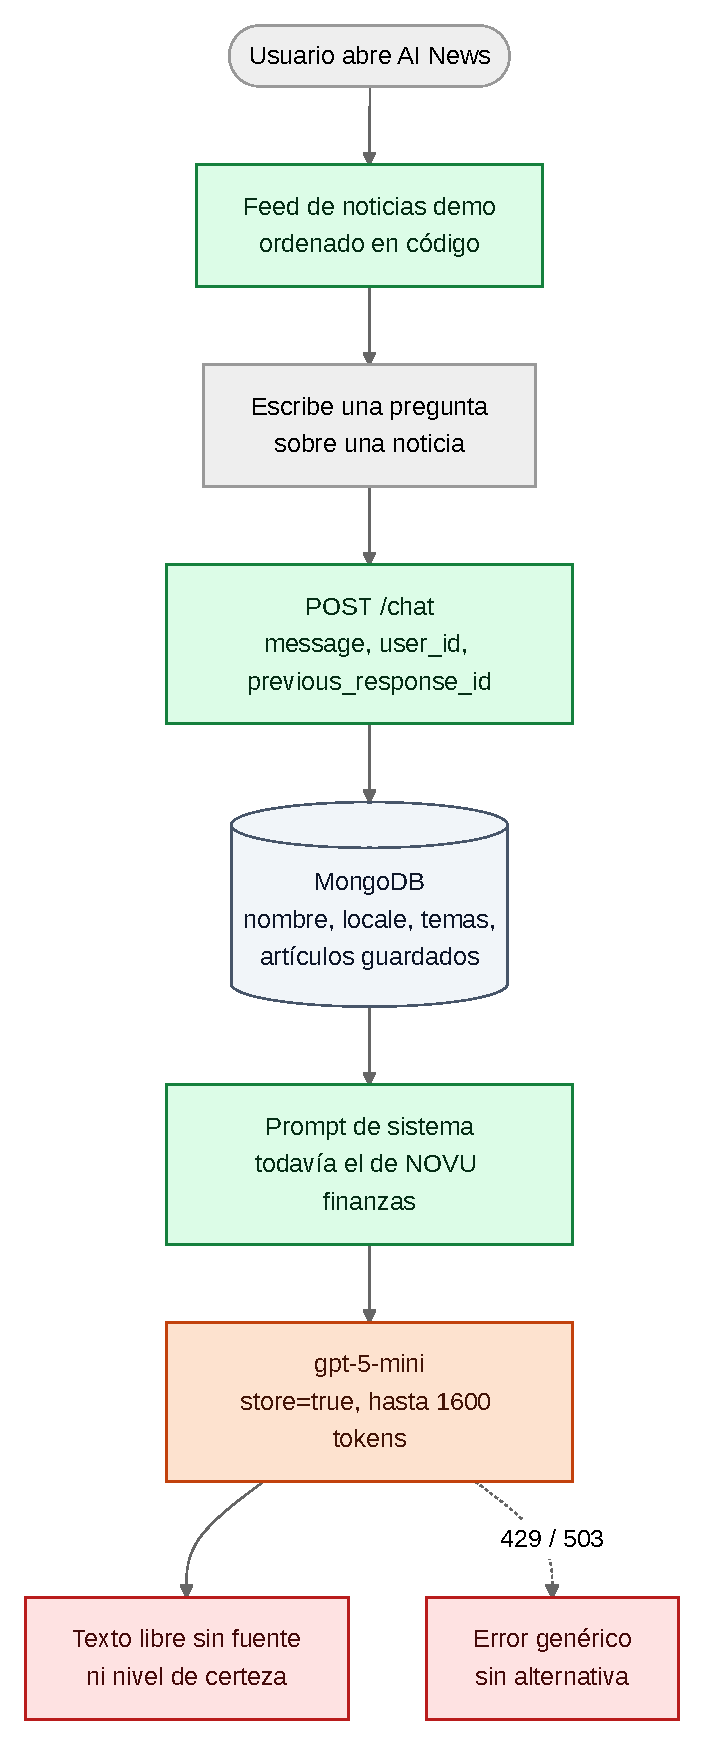
\includegraphics[width=\linewidth,height=190mm,keepaspectratio]{diagramas/flujo-actual.pdf}
  \raggedright
  \sub{Observado en el repositorio}
  \begin{itemize}
    \item Cada pregunta llega a gpt-5-mini, aunque sea una fecha o una fuente.
    \item Se envían nombre, locale y temas del usuario con cada turno.
    \item store=true: el historial queda en OpenAI.
    \item El prompt sigue siendo el de NOVU finanzas.
    \item La app móvil aún no tiene pantalla de chat; el feed usa datos demo.
  \end{itemize}
\end{panel}
\end{minipage}\hfill
\begin{minipage}[t]{0.215\linewidth}\vspace{0pt}
\begin{panel}[equal height group=f1]{2. Usuario y necesidad}
  \sub{Persona \HS}
  Estudiante o profesional joven en Guatemala. Lee noticias en el celular entre clases o en el bus, con datos móviles limitados.

  \sub{Necesidad}
  Entender rápido una noticia y saber si lo que lee está en la fuente o lo inventó la IA.

  \sub{Punto del flujo a mejorar}
  El momento después de escribir la pregunta: hoy espera varios segundos un texto sin cita y sin señal de duda.

  \sub{Qué cambia en la experiencia}
  \begin{itemize}
    \item Sugerencias tocables para lo frecuente: fecha, fuente, resumen.
    \item Los datos puntuales llegan como cita del párrafo, resaltada en la noticia.
    \item La IA generativa queda para explicar contexto y se etiqueta como tal.
    \item Cuando el sistema duda, lo dice y ofrece una salida.
  \end{itemize}

  \sub{Cómo se mantiene el valor}
  La persona sigue obteniendo respuesta en lenguaje natural y gana trazabilidad: puede ver de qué párrafo sale cada dato.
\end{panel}
\end{minipage}\hfill
\begin{minipage}[t]{0.55\linewidth}\vspace{0pt}
\begin{panel}[equal height group=f1]{3. Investigación: qué es Jev y qué implica usarlo}
\begin{minipage}[t]{0.325\linewidth}
  \sub{Tareas y límites frente a un LLM}
  Jev 1.13 recibe un estado en texto y preguntas tipadas. Devuelve respuestas con probabilidad y confianza en una sola llamada.
  \begin{itemize}
    \item Choice: elegir una opción de una lista.
    \item Score: calificar contra niveles de una rúbrica.
    \item Noul: probabilidad de que una afirmación sea verdadera.
  \end{itemize}
  Sirve para clasificar, enrutar, filtrar pasajes, verificar citas y extraer seleccionando entre candidatos.

  Límites documentados por TypeSafe:
  \begin{itemize}
    \item No genera texto ni conversa.
    \item Falla en conteo, aritmética y comparación de fechas.
    \item Lee las instrucciones de forma literal.
    \item Pierde precisión con estados grandes o con contenido adversarial.
    \item Sólo texto; 64k tokens por solicitud.
    \item Entrenado sobre todo en inglés; en español la precisión es menor.
  \end{itemize}
\end{minipage}\hfill
\begin{minipage}[t]{0.325\linewidth}
  \sub{Datos enviados y políticas}
  Enviaríamos la pregunta sin datos personales y párrafos de la noticia, que es contenido público. No enviaríamos user\_id, nombre, correo ni preferencias.

  \begin{itemize}
    \item Entrenamiento: la política de privacidad dice que no entrenan ni ajustan modelos con el input. \HV
    \item Conservación: mientras sea razonablemente necesario; sin plazo fijo. Retención cero sólo para empresas. \HV
    \item Ubicación: servicio alojado en EE. UU. \HV
    \item Terceros: comparten input sólo con proveedores de servicio; lista de subencargados en el DPA. \HV
    \item Telemetría: el sitio usa cookies y Google Analytics y registra IP, dispositivo y horarios. No encontramos qué registra la API por solicitud. \HS
    \item Acceso temprano por lista de espera; límites de uso cambian sin aviso. \HV
  \end{itemize}
\end{minipage}\hfill
\begin{minipage}[t]{0.325\linewidth}
  \sub{Velocidad, costo y recursos}
  \begin{itemize}
    \item Jev: US\$0.042 por millón de tokens de entrada; la salida no se cobra. \HV
    \item gpt-5-mini: US\$0.25 entrada y US\$2.00 salida por millón. \HV
    \item Límite Jev: 100k tokens/s y 40 solicitudes/s. \HV
    \item 193.6x más rápido y 444.6x más barato que un LLM; 0.114 s frente a 8.566 s. Prueba interna sin método publicado. \HP
    \item 13 preguntas en una llamada: 0.27 s y US\$0.0005, frente a 2.71 s con 13 llamadas. \HP
    \item Cero alucinaciones: válido sólo porque elige entre opciones dadas; puede elegir mal. \HP
    \item Energía o hardware por solicitud: no publicado. \HS
    \item Nuestros tiempos y costos por turno son estimaciones (ver panel 6). \HS
  \end{itemize}
\end{minipage}
\end{panel}
\end{minipage}

\vspace{10pt}

% ---------- Fila 2: matriz ----------
\begin{panel}{4. Matriz por función del flujo}
\renewcommand{\arraystretch}{1.35}
\fontsize{14}{18}\selectfont
\begin{tabularx}{\linewidth}{@{}>{\raggedright}p{75mm}>{\centering}p{25mm}>{\raggedright}X>{\raggedright}p{88mm}>{\raggedright}p{80mm}>{\raggedright}p{58mm}>{\raggedright}p{70mm}>{\raggedright\arraybackslash}p{88mm}@{}}
{\color{gris}Función} & {\color{gris}Elección} & {\color{gris}Justificación} & {\color{gris}UX} & {\color{gris}Privacidad} & {\color{gris}Velocidad} & {\color{gris}Costo y recursos} & {\color{gris}Funcionalidad} \\\hline
Mostrar fecha, fuente y enlace & \CODE & Son metadatos del artículo; ningún modelo agrega valor. & Respuesta inmediata y exacta. & No sale nada. & Instantáneo. & Nulo. & Igual. \\\hline
Mostrar resumen & \CODE & La fuente ya trae summary; si falta, se genera una vez y se guarda. & Disponible al tocar, sin espera. & No sale nada. & Instantáneo. & Una llamada por artículo, no por usuario. & Igual. \\\hline
Quitar datos personales de la pregunta & \CODE & Expresiones regulares para correos, teléfonos y DPI; Jev falla con números. & Invisible. & Menos exposición a terceros. & Milisegundos. & Nulo. & Puede omitir datos escritos de forma inusual. \\\hline
Clasificar la intención & \JEV & Choice entre cinco intenciones; la confianza decide la ruta. & Ruta adecuada sin preguntar al usuario. & Pregunta y noticia salen a TypeSafe. & Menos de un segundo. \HP & Fracción de centavo. & Menor precisión en español; se mitiga con umbral. \\\hline
Localizar el párrafo que responde & \JEV & Choice sobre párrafos numerados y Noul ¿la noticia contiene la respuesta? & Cita verificable en lugar de texto libre. & Misma llamada. & Misma llamada. & Misma llamada. & No puede combinar datos de varios párrafos. \\\hline
Detectar tema fuera de alcance o sensible & \JEV & Noul para consejo médico, legal o financiero personal. & Mensaje claro en lugar de una respuesta riesgosa. & Misma llamada. & Misma llamada. & Misma llamada. & Literal; necesita criterios explícitos. \\\hline
Decidir la ruta con umbrales & \CODE & El código controla las acciones; Jev sólo informa. & Comportamiento predecible. & No sale nada. & Instantáneo. & Nulo. & Umbrales ajustables por versión de Jev. \\\hline
Calcular hace cuánto pasó & \CODE & Jev compara fechas mal; la aritmética va en código. & Dato correcto. & No sale nada. & Instantáneo. & Nulo. & Igual. \\\hline
Explicar contexto o causas & \LLM & Requiere redactar; Jev no genera texto. & Respuesta rica, etiquetada como generada. & Sólo pregunta y párrafos relevantes; store=false. & Segundos. \HS & Mayor costo; sólo en esta ruta. & Puede inventar; se muestra la fuente al lado. \\\hline
Historial de la conversación & \CODE & Guardarlo en nuestra MongoDB en vez de previous\_response\_id. & Igual. & El historial no queda en OpenAI. & Igual. & Almacenamiento propio. & Igual. \\
\end{tabularx}
\end{panel}

\vspace{10pt}

% ---------- Fila 3: flujo propuesto, datos, Responsible AI ----------
\begin{minipage}[t]{0.335\linewidth}\vspace{0pt}
\begin{panel}[equal height group=f3]{5. Flujo propuesto}
  \centering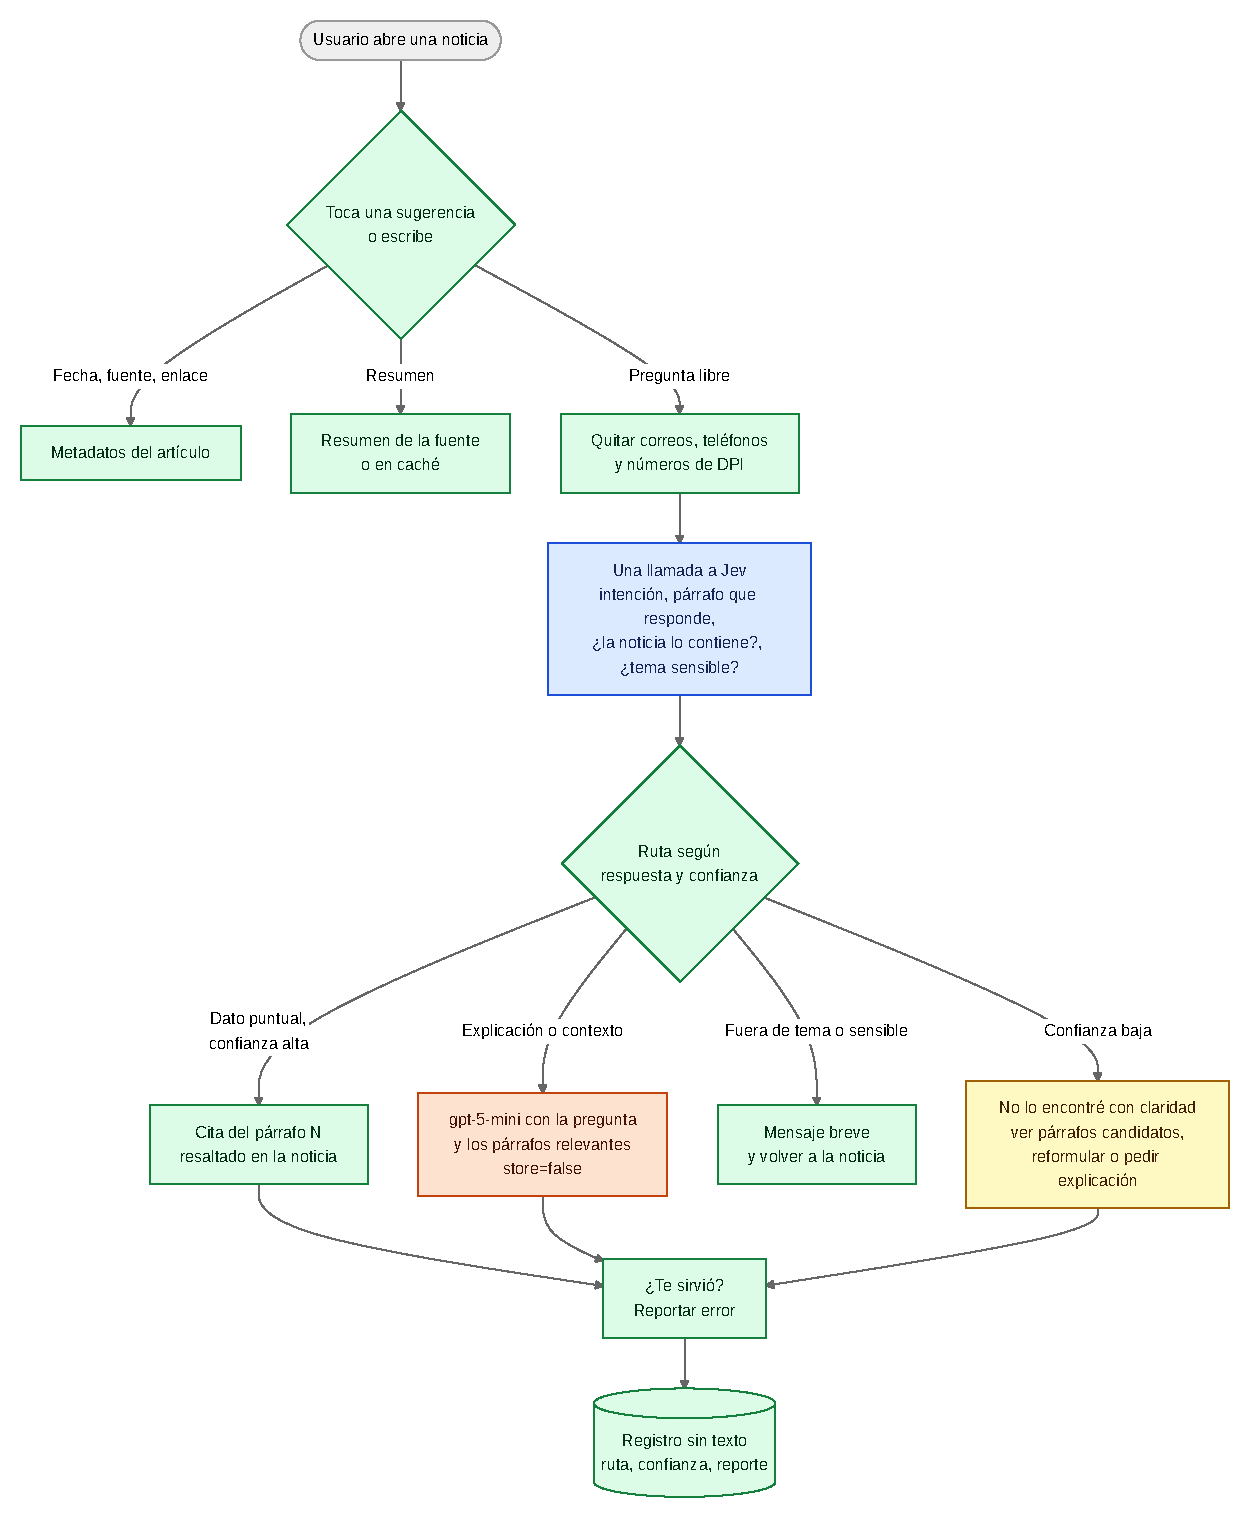
\includegraphics[width=\linewidth,height=240mm,keepaspectratio]{diagramas/flujo-propuesto.pdf}
\end{panel}
\end{minipage}\hfill
\begin{minipage}[t]{0.31\linewidth}\vspace{0pt}
\begin{panel}[equal height group=f3]{6. Datos que salen y comparación Lean}
  \centering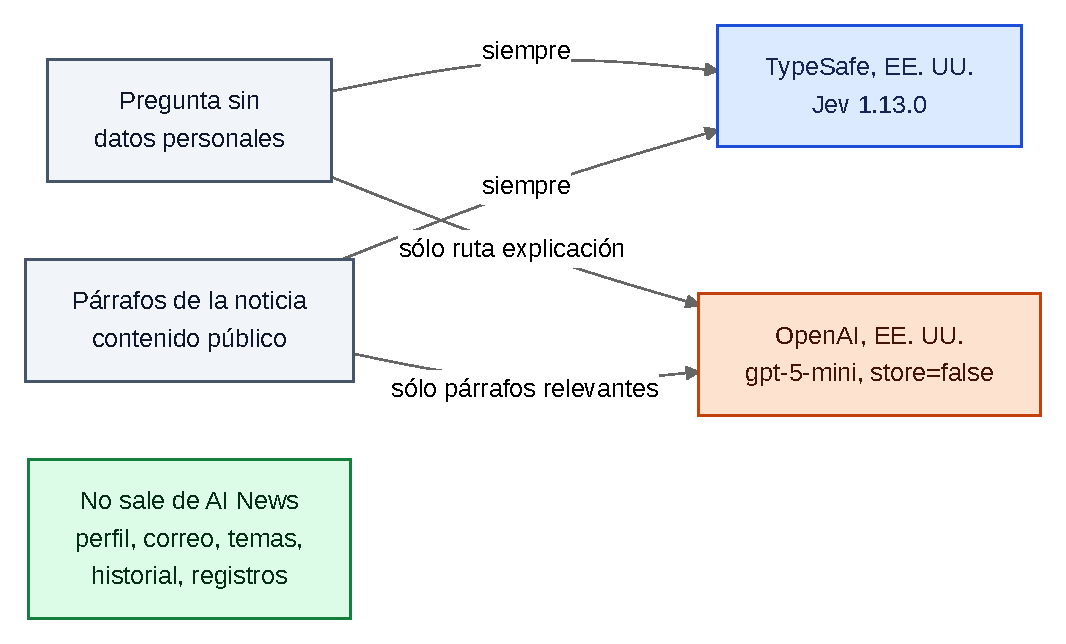
\includegraphics[width=\linewidth,height=80mm,keepaspectratio]{diagramas/datos.pdf}
  \raggedright
  \sub{Llamadas que aportan valor y llamadas evitables}
  Hoy hay una llamada al LLM por cada pregunta. Fecha, fuente y resumen no la necesitan. Las preguntas de dato puntual se resuelven con una cita. El LLM queda para explicar.

  \sub{Costo por 1000 preguntas \HS}
  \fontsize{14}{18}\selectfont\renewcommand{\arraystretch}{1.3}
  \begin{tabularx}{\linewidth}{@{}>{\raggedright}X>{\raggedleft}p{30mm}>{\raggedleft\arraybackslash}p{30mm}@{}}
    {\color{gris}Supuesto} & {\color{gris}Actual} & {\color{gris}Propuesto} \\\hline
    Llamadas a gpt-5-mini & 1000 & 400 \\
    Tokens entrada / salida LLM & 2000 / 400 & 1200 / 400 \\
    Llamadas a Jev, 1500 tokens & 0 & 1000 \\
    Costo LLM & US\$1.30 & US\$0.44 \\
    Costo Jev & 0 & US\$0.06 \\\hline
    Total & US\$1.30 & US\$0.50 \\
  \end{tabularx}
  \fontsize{15}{19.5}\selectfont
  \par\vspace{4pt}
  Se asume que 60\% de las preguntas son dato puntual, metadatos o fuera de tema. La salida del LLM incluye tokens de razonamiento.

  \sub{Qué se gana y qué se pierde}
  Se gana latencia, costo y trazabilidad. Se pierde flexibilidad en preguntas ambiguas, se agrega un proveedor y aparece un caso nuevo de error: una mala ruta.
\end{panel}
\end{minipage}\hfill
\begin{minipage}[t]{0.335\linewidth}\vspace{0pt}
\begin{panel}[equal height group=f3]{7. Medidas de Responsible AI}
  \sub{Datos mínimos}
  A Jev: pregunta sin datos personales y párrafos numerados. Al LLM: lo mismo, sólo en la ruta de explicación. Perfil, correo, temas e historial no salen. Se fija la versión jev-1.13.0 para que las respuestas no cambien sin aviso.

  \sub{Límites e incertidumbre}
  \begin{itemize}
    \item Etiqueta en cada respuesta: Extraído del párrafo N o Explicación generada por IA, puede contener errores.
    \item Confianza baja: No lo encontré con claridad en la noticia, con párrafos candidatos y opciones para seguir.
    \item No se muestran porcentajes crudos; se usan tres estados: seguro, revisar, no encontrado.
  \end{itemize}

  \sub{Si la decisión es incorrecta}
  La cita permite verificar en la noticia. El botón No responde mi pregunta pasa a la explicación del LLM o permite reformular. Cada reporte guarda ruta, confianza y versión, sin el texto, y se revisa cada semana para ajustar umbrales.

  \sub{Riesgo de sesgo o exclusión}
  Jev rinde mejor en inglés. Quien escribe en español coloquial guatemalteco, con voseo, errores de ortografía o con el español como segunda lengua recibiría más rutas equivocadas y más respuestas de no encontrado.

  \sub{Medida concreta}
  Antes de lanzar: 150 preguntas reales en español guatemalteco etiquetadas, con precisión medida por grupo. Si la precisión de un grupo queda bajo 85\%, su ruta por defecto es el LLM. En confianza baja se ofrecen sugerencias tocables en lugar de pedir que reescriba.
\end{panel}
\end{minipage}

\vspace{10pt}

% ---------- Fila 4: conclusión, supuestos, fuentes ----------
\begin{minipage}[t]{0.25\linewidth}\vspace{0pt}
\begin{panel}[equal height group=f4]{8. Conclusión}
  Arquitectura híbrida con el código al mando. Metadatos, resumen, filtros, fechas y rutas van en código. Jev toma las decisiones cerradas con una sola llamada por pregunta. El LLM sólo redacta cuando hay que explicar, con menos datos y sin guardar historial en el proveedor.

  La persona recibe respuestas más rápidas, con cita y con un aviso cuando el sistema no está seguro.
\end{panel}
\end{minipage}\hfill
\begin{minipage}[t]{0.35\linewidth}\vspace{0pt}
\begin{panel}[colback=supf,colframe=sup!50,equal height group=f4]{9. Supuestos y lo que falta verificar}
  \begin{itemize}
    \item Persona y necesidad: sin entrevistas; validar con 5 usuarios.
    \item Distribución de preguntas y tokens por turno: medir con registros reales.
    \item Latencia de Jev desde Guatemala y precisión en español: probar en el Playground.
    \item Qué registra la API por solicitud y plazo de conservación: preguntar a TypeSafe.
    \item Términos del Master Customer Agreement para uso por API.
    \item Disponibilidad: acceso temprano con lista de espera.
    \item Umbral de 85\% y tamaño de 150 preguntas: valores iniciales a revisar.
  \end{itemize}
\end{panel}
\end{minipage}\hfill
\begin{minipage}[t]{0.38\linewidth}\vspace{0pt}
\begin{panel}[equal height group=f4]{10. Fuentes consultadas}
  \fontsize{12.5}{16}\selectfont
  \begin{itemize}
    \item Documentación Jev: \url{https://docs.typesafe.ai/introduction}
    \item Modelos, precio, límites, idiomas: \url{https://docs.typesafe.ai/models}
    \item Límites de jev-1.13: \url{https://docs.typesafe.ai/model-jaggedness/jev-1.13}
    \item Confianza: \url{https://docs.typesafe.ai/confidence}
    \item Preguntas en paralelo: \url{https://docs.typesafe.ai/cookbooks/parallel_questions}
    \item Legal y retención cero: \url{https://docs.typesafe.ai/legal}
    \item Política de privacidad: \url{https://typesafe.ai/legal/privacy-policy}
    \item Data Processing Agreement: \url{https://typesafe.ai/legal/data-processing}
    \item Términos de uso: \url{https://typesafe.ai/legal/terms}
    \item Afirmaciones de velocidad y costo: \url{https://typesafe.ai}
    \item Precio gpt-5-mini: \url{https://developers.openai.com/api/docs/models/gpt-5-mini}
    \item Código del Proyecto 2: backend/assistant y frontend de ai-assisted-news-app
  \end{itemize}
  Consultadas el 30 de septiembre de 2026.
\end{panel}
\end{minipage}

\end{document}
